\begin{columns}[t]
\begin{column}{\sepwid}\end{column}\begin{column}{\onecolwid}

\begin{alertblock}{Design of Block Ciphers}
	\begin{center}
			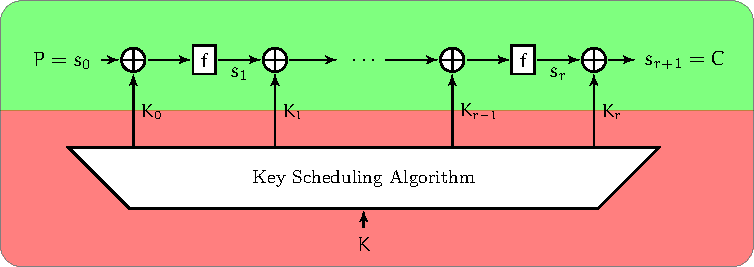
\includegraphics[keepaspectratio,width=\textwidth]{figures/motivation/plot.pdf}
	\end{center}

%	Design rationales for block ciphers are nowadays a thorough scrutinzed topic.
%	Properties of good S-boxes and strategies for secure linear layers are well understood.
%	Interestingly, when it comes to the key schedule, we know not anywhere near as much about its security implications.
%	Particularly, this crucial understudied topic might has an impact on security margins~\cite{C:AABL12}, especially in the case of lightweight cryptographic designs that utilises very simple key schedules.
%
%	With our work, we shed some light on the influences of key schedules and give a first result on sound design strategies for this important part of block ciphers.
\end{alertblock}

\begin{block}{Problem}
	\begin{itemize}
		\item Abdelraheem~et~al.\ (2012), cf.\ Fig.~1:\\
			\present/ with const.\ round keys is weaker than with indp.\ round keys.
		\item How do different S-boxes influence this behaviour?
		\item Interesting candidate: $R_1$, cf.\ Fig.~2.
		\item Its convergence distribution fulfills \emph{Tchebysheff's inequality tightly}.
	\end{itemize}
\end{block}

\end{column}
\begin{column}{\sepwid}\end{column}\begin{column}{\onecolwid}

\begin{block}{Experimental Setup}
	\begin{center}
		\begin{tikzpicture}

			\tikzstyle{every node}=[transform shape];

			% data path
			\node (XOR-1)[XOR,line width=3pt,scale=1.2,fill=white] {};
			\node [left=1em of XOR-1] (p) {$\langle \alpha, s_{0} \rangle$};
			\node (f-1) [right=2em of XOR-1,draw,rectangle,dashed,line width=3pt,fill=white,rounded corners] {\begin{tikzpicture}
					\node [draw,rectangle,solid,line width=3pt,fill=lichtgrau,rounded corners,text width=4cm,align=center] (s) {S-box Layer};
					\node [right=1em of s,draw,rectangle,solid,line width=3pt,fill=white,rounded corners,text width=4cm,align=center] (lin) {Linear Layer};
					\path[line,solid] (s) edge (lin);
				\end{tikzpicture}};
			\path[line] (p) edge (XOR-1);
			\path[line] (XOR-1) edge (f-1);
			\node(k-0) [above=2em of XOR-1,fill=lichtgrau,rounded corners] {\small $k_{0} \in_R \mathbb{F}_2^n$};
			\path[line] (k-0) edge (XOR-1);

			\node (XOR-2)[right=2em of f-1,XOR,line width=3pt,scale=1.2,fill=white] {};
			\node(k-1) [above=2em of XOR-2,fill=lichtgrau,rounded corners] {\small $k_{1} \in_R \mathbb{F}_2^n$};
			\path[line] (k-1) edge (XOR-2);

			\node(dots)[right=2em of XOR-2] {$\dots$};
			\node(c)[right=2em of dots] {$\langle \beta, s_{r+1} \rangle$};

			\path[line] (f-1) edge (XOR-2);
			\path[line] (XOR-2) edge (dots);
			\path[line] (dots) edge (c);

			\node(vs)[below=1em of XOR-1] {vs.};

			\node(XOR-11)[below=1em of vs,XOR,line width=3pt,scale=1.2,fill=white] {};
			\node(p1)[left=1em of XOR-11] {$\langle \alpha, s_{0} \rangle$};
			\node(f-11)[right=2em of XOR-11,draw,rectangle,dashed,line width=3pt,fill=white,rounded corners] {\begin{tikzpicture}
					\node(s1)[draw,rectangle,solid,line width=3pt,fill=lichtgrau,rounded corners,text width=4cm,align=center] {S-box Layer};
					\node(lin1)[right=1em of s1,draw,rectangle,solid,line width=3pt,fill=white,rounded corners,text width=4cm,align=center] {Linear Layer};
					\path[line,solid] (s1) edge (lin1);
				\end{tikzpicture}};
			\path[line] (p1) edge (XOR-11);
			\path[line] (XOR-11) edge (f-11);
			\node(k-01) [below=2em of XOR-11,fill=lichtgrau,rounded corners] {\small $k_{0} = k$};
			\path[line] (k-01) edge (XOR-11);

			\node (XOR-12)[right=2em of f-11,XOR,line width=3pt,scale=1.2,fill=white] {};
			\node(k-11) [below=2em of XOR-12,fill=lichtgrau,rounded corners] {\small $k_{1} = k$};
			\path[line] (k-11) edge (XOR-12);

			\node(dots1)[right=2em of XOR-12] {$\dots$};
			\node(c1)[right=2em of dots1] {$\langle \beta, s_{r+1} \rangle$};

			\path[line] (f-11) edge (XOR-12);
			\path[line] (XOR-12) edge (dots1);
			\path[line] (dots1) edge (c1);

		\end{tikzpicture}
	\end{center}
	\vspace{0.5em}
	\begin{center}
		What is the distribution of \begin{equation*}
				\text{Pr}\bracket*{\iprod{\alpha, s_0} = \iprod{\beta, s_{r+1}}}
			\end{equation*}
		over $k$ and the choice of the S-box?
	\end{center}
	\vspace{0.5em}
	\begin{center}
		\noindent\fcolorbox{lichtgrau}{lichtgrau}{\begin{minipage}{0.85\textwidth}
				\centering
				\vspace{1em}
				We cannot hope to prove better bounds than Tchebysheff\\
				in general for resistence against linear cryptanalysis.
				\vspace{1em}
		\end{minipage}}%
	\end{center}
\end{block}

\end{column}
\end{columns}

%----------------------------------------------------------------------------------------

\begin{columns}[t]
\begin{column}{\sepwid}\end{column}\begin{column}{\twocolwid}

\begin{block}{Experimental Results}
	\begin{minipage}{0.245\textwidth}
		\begin{figure}[ht!]
			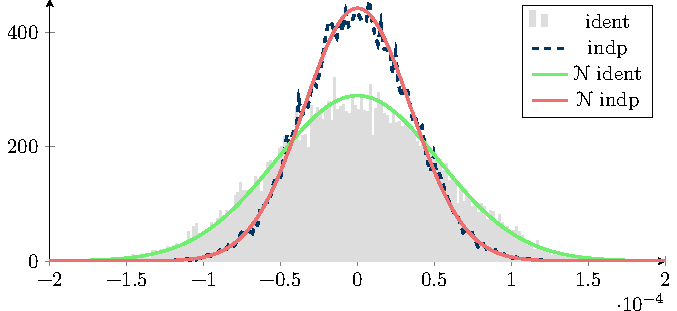
\includegraphics[keepaspectratio,width=\textwidth]{figures/distribution_present/plot.pdf}
			\caption{Standard \present/.}\label{fig:std_present}
		\end{figure}
	\end{minipage}
	\begin{minipage}{0.245\textwidth}
		\begin{figure}[ht!]
			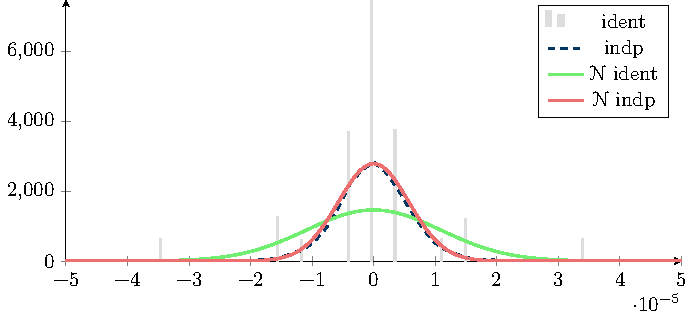
\includegraphics[keepaspectratio,width=\textwidth]{figures/distribution_r1/plot.pdf}
			\caption{\present/ with $R_1$ S-box.}\label{fig:present_r1}
		\end{figure}
	\end{minipage}
	\begin{minipage}{0.245\textwidth}
		\begin{figure}[ht!]
			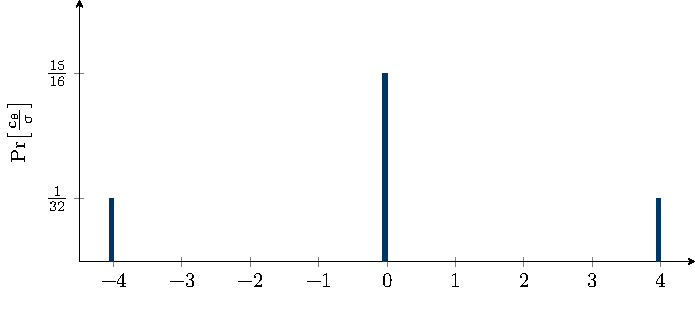
\includegraphics[keepaspectratio,width=\textwidth]{figures/distribution_convergence/plot.pdf}
			\caption{Convergence distribution.}\label{fig:convergence}
		\end{figure}
	\end{minipage}
	\begin{minipage}{0.245\textwidth}
		\begin{figure}[ht!]
			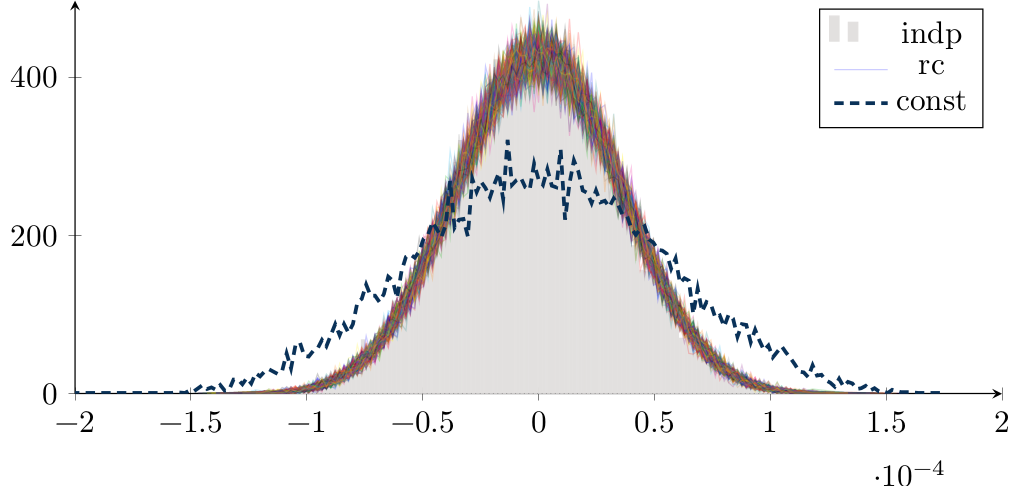
\includegraphics[keepaspectratio,width=\textwidth]{figures/distribution_rc/plot.png}
			\caption{Influence of round constants.}\label{fig:rc}
		\end{figure}
	\end{minipage}
\end{block}

\end{column}
\end{columns}

%----------------------------------------------------------------------------------------

\begin{columns}[t]
\begin{column}{\sepwid}\end{column}\begin{column}{\onecolwid}

\begin{block}{How to Design a Key Schedule:}
	Typically, a design uses round constants to avoid slide attacks, etc., and break symmetries in the round function.
	\vspace{0.5em}
	\begin{center}
		\noindent\fcolorbox{lichtgrau}{lichtgrau}{\begin{minipage}{0.85\textwidth}
				\centering
				\vspace{1em}
				To design a good key schedule against linear cryptanalysis, it is\\
				on average sufficient to choose any linear key schedule $L_i$ and fix\\
				randomly chosen round constants $c_i$.
				\vspace{1em}
		\end{minipage}}%
	\end{center}
	\vspace{1em}
	\begin{equation*}
		\mathbb{E}_c\parens{\text{Var}\parens{\widehat{E_k}\parens{\alpha, \beta}}} = 2^{-n\parens{r+1}} \sum_c \F_2^{-\ell} \sum_{k \in \F_2^\ell} \widehat{E_k}\parens*{\alpha,\beta}^2 = 2^{2n} \sum_{\tower{\gamma}{\gamma_0 = \alpha, \gamma_r = \beta}} C_\gamma^2
	\end{equation*}
\end{block}

\end{column}
\begin{column}{\sepwid}\end{column}\begin{column}{\onecolwid}

\begin{block}{Round Constants}
	\vspace{3em}
	\begin{center}
		\begin{tikzpicture}
			\tikzstyle{every node}=[transform shape];

			% data path
			\node (XOR-1)[XOR,line width=3pt,scale=1.2,fill=white] {};
			\node [left=1em of XOR-1] (p) {$\langle \alpha, s_{0} \rangle$};
			\node (f-1) [right=2em of XOR-1,draw,rectangle,dashed,line width=3pt,fill=white,rounded corners] {\begin{tikzpicture}
					\node [draw,rectangle,solid,line width=3pt,fill=white,rounded corners,text width=4cm,align=center] (s) {S-box Layer};
					\node [right=1em of s,draw,rectangle,solid,line width=3pt,fill=white,rounded corners,text width=4cm,align=center] (lin) {Linear Layer};
					\path[line,solid] (s) edge (lin);
				\end{tikzpicture}};
			\path[line] (p) edge (XOR-1);
			\path[line] (XOR-1) edge (f-1);
			\node(k-0) [above=2em of XOR-1,fill=lichtgrau,rounded corners] {\small $L_0(k)$};
			\node(c-0) [below=2em of XOR-1,fill=lichtgrau,rounded corners] {\small $c_0$};
			\path[line] (k-0) edge (XOR-1);
			\path[line] (c-0) edge (XOR-1);

			\node(XOR-2)[right=2em of f-1,XOR,line width=3pt,scale=1.2,fill=white] {};
			\node(k-1) [above=2em of XOR-2,fill=lichtgrau,rounded corners] {\small $L_1(k)$};
			\node(c-1) [below=2em of XOR-2,fill=lichtgrau,rounded corners] {\small $c_1$};
			\path[line] (k-1) edge (XOR-2);
			\path[line] (c-1) edge (XOR-2);
			\path[line] (f-1) edge (XOR-2);

			\node(dots)[right=2em of XOR-2] {$\dots$};
			\node(c)[right=2em of dots] {$\langle \beta, s_{r+1} \rangle$};

			\path[line] (XOR-2) edge (dots);
			\path[line] (dots) edge (c);
		\end{tikzpicture}
	\end{center}
	%\vspace{1em}
	%In fact, choosing any linear key schedule and random round constants is, \emph{on average}, as good as having independent round keys and thus a sound design decision (cf.~Fig.~4 for experimental verification):
\end{block}

\end{column}
\end{columns}

%----------------------------------------------------------------------------------------

\begin{columns}[t]
\begin{column}{\smallsepwid}\end{column}\begin{column}{\twocolwid}
\setbeamercolor{block alerted title}{fg=saphierblau,bg=lichtgrau}
\setbeamercolor{block alerted body}{fg=black,bg=white}

\begin{alertblock}{Background}
	\begin{columns}[t]
	\begin{column}{0.001\paperwidth}\end{column}\begin{column}{\smallonecolwid}

	\begin{block}{Linear Cryptanalysis}
%		\begin{center}
%			\textbf{\color{saphierblau}{Linear Cryptanalysis}}\\[1em]
%		\end{center}
		For a block cipher $E_k : \F_2^n \to \F_2^m$, we need to find good \emph{input/output masks} $\parens*{\alpha, \beta} \in \F_2^n \times \F_2^m$, s.\,t. $\iprod{\alpha, x} = \iprod{\beta, E_k\parens*{x}}$ holds for many $x$.
		The Fourier coefficient $\widehat{E_k}$ at the point $\parens*{\alpha, \beta}$ is
		$\widehat{E_k}\parens*{\alpha, \beta} := \sum_{x \in \F_2^n} \parens*{-1}^{\iprod{\alpha, x} + \iprod{\beta, E_k\parens*{x}}}$.
		%In our experiments, we use the \emph{correlation} $c_{E_k}\parens*{\alpha, \beta}$, which is a scaled notation: $2^n c_{E_k}\parens*{\alpha, \beta} = \widehat{E_k}\parens*{\alpha, \beta}$.

		%Nyberg showed that for \emph{any} $F: \F_2^n \times \F_2^\ell \to \F_2^m$, $E_k(x) := F(x, k)$:
		%\begin{equation*}
		%	2^\ell \widehat{E_k}\parens*{\alpha, \beta} = \sum_{\theta \in \F_2^\ell} \parens*{-1}^{\iprod{\theta, k}}\widehat{F}\parens*{\parens*{\alpha,\theta}, \beta}.
		%\end{equation*}
		%Thus, correlations exhibit a key dependent behaviour.
		%In the case of $F$ being a key alternating block cipher with $(r+1)$ independent round keys ($\textsf{KeyAlt}_{Id}$), we can write this as
		%\begin{equation*}
		%	\widehat{E_k}(\alpha,\beta) = 2^{-n(r+1)}\sum_{\theta \in \F_2^\ell} \parens*{-1}^{\iprod{\theta,k}}\widehat{\textsf{KeyAlt}_{Id}}((\alpha,\theta),\beta)
		%	= 2^n\sum_{\tower{\gamma}{\gamma_0 = \alpha,\gamma_r=\beta}} \parens*{-1}^{\iprod{\gamma,k}}  C_{\gamma}.
		%\end{equation*}
		%This is the well known linear hull.
	\end{block}

	\end{column}
	\begin{column}{\smallsepwid}\end{column}\begin{column}{\smallonecolwid}

%	\vspace*{1em}
	\begin{block}{\present/~(Bogdanov~et~al.\ 2007)}
%	\begin{center}
%		\textbf{\color{saphierblau}{\present/~(Bogdanov~et~al.\ 2007)}}\\[1em]
%	\end{center}
		\begin{minipage}{0.329\smallonecolwid}
			\begin{itemize}
				\item lightweight block cipher
				\item one bit trails dominate\\(Ohkuma 2009)
			\end{itemize}
		\end{minipage}
		\hspace*{15mm}
		\begin{minipage}{0.32\smallonecolwid}
			\begin{itemize}
				\item SPN with 64~bit blocks
				\item[] \vphantom{empty line}
			\end{itemize}
		\end{minipage}
		\hspace*{15mm}
		\begin{minipage}{0.225\smallonecolwid}
			\begin{itemize}
				\item 4~bit S-box
				\item Bitpermutation\\\vphantom{empty line}
			\end{itemize}
		\end{minipage}
	\end{block}

	\end{column}
	\end{columns}

\end{alertblock}

\end{column}
\end{columns}

%----------------------------------------------------------------------------------------

\begin{columns}[t]
\begin{column}{\sepwid}\end{column}\begin{column}{\onecolwid}

\setbeamercolor{block title}{fg=ucorange,bg=white} % Change the block title color
\begin{block}{Acknowledgements}
	\small{\rmfamily{This work was supported by the DFG Research Training Group GRK 1817 UbiCrypt.}} \\
	\vspace{1cm}
\end{block}

\end{column}
\begin{column}{\sepwid}\end{column}\begin{column}{\onecolwid}

\setbeamercolor{block title}{fg=saphierblau,bg=white}
\begin{block}{References}
	\nocite{*}
	\printbibliography{}
\end{block}

\end{column}
\end{columns}
